

\section{HU2 Pantalla de registro de alumno}

En esta pantalla en Actor tendrá que rellenar los campos solicitados, Nombre, Primer Apellido, Segundo Apellido y matricula.\\
Botón: regresar- regresa a la pantalla HU1 Pantalla de inicio.\\
Botón: limpiar-limpia todos los campos dejandolos vacios.\\
Botón: registrar-termina el registro.
\begin{figure}[h]
	\centering
	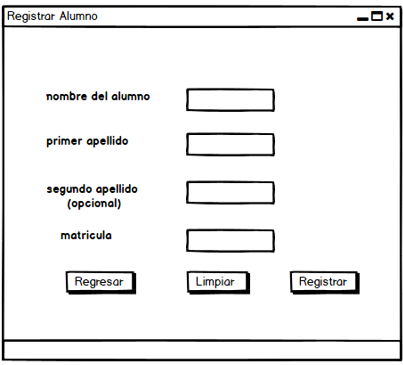
\includegraphics[scale=0.5]{./HistoriasUsuario/imagenes/IHU2.png}
	\caption{Pantalla de registro de alumno}
\end{figure}
Si no se llenan los campos que deben ser obligatorios aparecerá la siguiente leyenda debajo de cada campo indicando con un  “ * “ los campos obligatorios.
\begin{figure}[h]
	\centering
	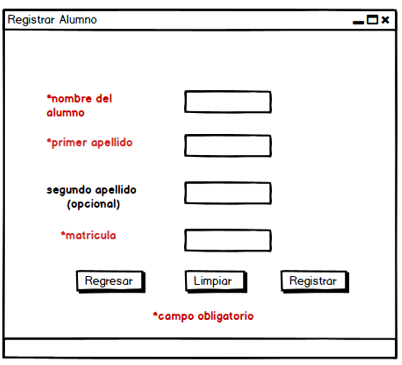
\includegraphics[scale=0.5]{./HistoriasUsuario/imagenes/IHU3.png}
	\caption{Pantalla campos obligatorios}
\end{figure}
Una vez registrado el alumno aparecerá el siguiente mensaje:
\begin{figure}[h]
	\centering
	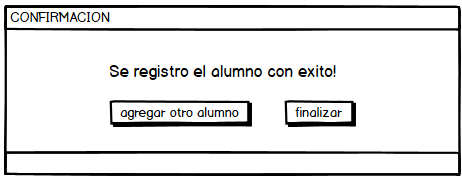
\includegraphics[scale=0.5]{./HistoriasUsuario/imagenes/IHU4.png}
	\caption{Pantalla mensaje de confirmación}
\end{figure}
Si se desea agregar otro alumno únicamente selecciona el botón “agregar otro alumno” y lo regresara a la pantalla de la figura 4.2 Pantalla de registro de alumno
Después de darle en “finalizar” le aparecerá la pantalla principal como se muestra en la figura 4.1 Pantalla de inicio de aplicación.
\begin{figure}[h]
	\centering
	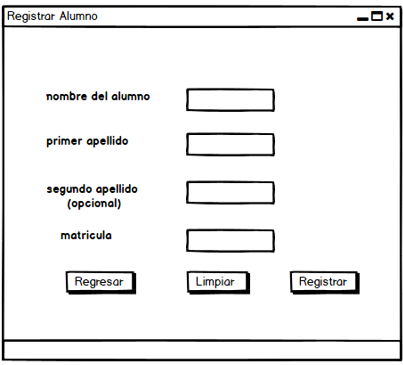
\includegraphics[scale=0.5]{./HistoriasUsuario/imagenes/IHU2.png}
\end{figure}
